% Options for packages loaded elsewhere
\PassOptionsToPackage{unicode}{hyperref}
\PassOptionsToPackage{hyphens}{url}
%
\documentclass[
  10pt,
  a4paper,
]{article}
\usepackage{amsmath,amssymb}
\usepackage{iftex}
\ifPDFTeX
  \usepackage[T1]{fontenc}
  \usepackage[utf8]{inputenc}
  \usepackage{textcomp} % provide euro and other symbols
\else % if luatex or xetex
  \usepackage{unicode-math} % this also loads fontspec
  \defaultfontfeatures{Scale=MatchLowercase}
  \defaultfontfeatures[\rmfamily]{Ligatures=TeX,Scale=1}
\fi
\usepackage{lmodern}
\ifPDFTeX\else
  % xetex/luatex font selection
\fi
% Use upquote if available, for straight quotes in verbatim environments
\IfFileExists{upquote.sty}{\usepackage{upquote}}{}
\IfFileExists{microtype.sty}{% use microtype if available
  \usepackage[]{microtype}
  \UseMicrotypeSet[protrusion]{basicmath} % disable protrusion for tt fonts
}{}
\makeatletter
\@ifundefined{KOMAClassName}{% if non-KOMA class
  \IfFileExists{parskip.sty}{%
    \usepackage{parskip}
  }{% else
    \setlength{\parindent}{0pt}
    \setlength{\parskip}{6pt plus 2pt minus 1pt}}
}{% if KOMA class
  \KOMAoptions{parskip=half}}
\makeatother
\usepackage{xcolor}
\usepackage[margin=25mm]{geometry}
\usepackage{longtable,booktabs,array}
\usepackage{calc} % for calculating minipage widths
% Correct order of tables after \paragraph or \subparagraph
\usepackage{etoolbox}
\makeatletter
\patchcmd\longtable{\par}{\if@noskipsec\mbox{}\fi\par}{}{}
\makeatother
% Allow footnotes in longtable head/foot
\IfFileExists{footnotehyper.sty}{\usepackage{footnotehyper}}{\usepackage{footnote}}
\makesavenoteenv{longtable}
\usepackage{graphicx}
\makeatletter
\def\maxwidth{\ifdim\Gin@nat@width>\linewidth\linewidth\else\Gin@nat@width\fi}
\def\maxheight{\ifdim\Gin@nat@height>\textheight\textheight\else\Gin@nat@height\fi}
\makeatother
% Scale images if necessary, so that they will not overflow the page
% margins by default, and it is still possible to overwrite the defaults
% using explicit options in \includegraphics[width, height, ...]{}
\setkeys{Gin}{width=\maxwidth,height=\maxheight,keepaspectratio}
% Set default figure placement to htbp
\makeatletter
\def\fps@figure{htbp}
\makeatother
\setlength{\emergencystretch}{3em} % prevent overfull lines
\providecommand{\tightlist}{%
  \setlength{\itemsep}{0pt}\setlength{\parskip}{0pt}}
\setcounter{secnumdepth}{-\maxdimen} % remove section numbering
\AtBeginDocument{\hypersetup{pdftitle={Supplementary material v9: Governance delay and the stability of harvested stocks},pdfauthor={Amin Abaee},pdfsubject={RFDE Hopf verification, protective review stability, nonlinear stock floors and institutional event evidence},pdfkeywords={delay differential equations, institutional feedback, sampled-data control, small-gain stability, harvested stocks, Hopf bifurcation, regime shifts}}}
\ifLuaTeX
  \usepackage{selnolig}  % disable illegal ligatures
\fi
\usepackage{bookmark}
\IfFileExists{xurl.sty}{\usepackage{xurl}}{} % add URL line breaks if available
\urlstyle{same}
\hypersetup{
  hidelinks,
  pdfcreator={LaTeX via pandoc}}

\author{}
\date{}

\begin{document}

\section{Supplementary Material: Governance Delay and Institutional
Feedback}\label{supplementary-material-governance-delay-and-institutional-feedback}

\textbf{Amin Abaee} · \href{https://orcid.org/0000-0002-0019-1842}{ORCID
0000-0002-0019-1842}\\
Governance manuscript v42; supplementary material v9 · 29 October 2026

This supplement gives the equations, proofs, numerical protocols and
evidence supporting the main article. Local nonlinear Hopf hypotheses
and protective review/viability inequalities are distinguished from
finite-dimensional fold certificates, floating periodic-orbit evidence
and observational event-clock constraints. S1--S12 contain the core
methods and model comparisons; S13--S16 give the nonlinear normal-form
derivation, all-cadences and stock-floor details, connected-branch
evidence and institutional-event protocol.

\textbf{Notation.} We use the symbols of the main article. The state
variables are the stock \(N\), the institutional memory \(Z\), and the
deployed effort \(E\). The mobilising and protective feedback channels
carry linearised coefficients \((C_E, C_Z)\) with subscripted variants
for the two channels. The delay \(\tau\) is deployment latency; \(T_r\)
is periodic review cadence. Governance capital, when introduced in S4.4,
is \(K_{\mathrm{cap}}\), not \(Z\). The candidate parameter sets A and B
and the four-state working core are as in the main article. The
following terms recur throughout and are glossed here on first use: an
\emph{interval Newton method} is a validated-root enclosure technique
that returns a rigorous box containing any root of a system in a
declared interval; a \emph{Krawczyk inclusion} is a validated interval
enclosure constructed from the Krawczyk operator; a \emph{Moore--Spence
system} is the standard augmented system for fold computation; a
\emph{radii polynomial} is a constructive validation tool for
infinite-dimensional problems; a \emph{Floquet multiplier} is an
eigenvalue of the monodromy map for a periodic orbit; a \emph{Hopf
enclosure} is an interval that contains the bifurcation delay with
rigorous outward rounding; and \emph{collocation} denotes a Fourier
Galerkin discretisation of the periodic-orbit boundary-value problem.

\begin{center}\rule{0.5\linewidth}{0.5pt}\end{center}

\subsection{S1. Interval Hopf
Enclosures}\label{s1.-interval-hopf-enclosures}

This section gives the validated enclosures for the delays at which the
gated Candidate A equilibrium changes linear stability. The enclosures
underwrite the qualitative Hopf statement of the main article; they do
not, by themselves, amount to a validated Hopf bifurcation theorem. That
distinction is preserved as the scope paragraph S1.3 below.

\textbf{Definition S1.1} (Cubic and phase relation). With
\(P(\lambda) = (\lambda - A_N)(\lambda + d)(\lambda - C_E)\) and
\(L(\lambda) = B_E(\lambda - A_N) + A_E B_N\), the modulus condition of
Theorem 4.1 of the main article gives the explicit cubic
\[H(x) = (x + A_N^2)(x + d^2)(x + C_E^2) - C_Z^2\bigl[B_E^2 x + (A_E B_N - A_N B_E)^2\bigr],\]
and at the interior equilibrium of the gated core the filter identity
\(A_E B_N - A_N B_E = 0\) reduces it to
\(H(x) = (x + A_N^2)(x + d^2)(x + C_E^2) - C_Z^2 B_E^2 x\). The delay is
the interval evaluation of the phase relation
\(\tau(\omega) = (-\arg(P(i\omega)/(C_Z L(i\omega))) + 2\pi k)/\omega\)
at a certified positive root of \(H\), not a root of an argument
formula.

\textbf{Proposition S1.2} (Certified enclosures, gated Candidate A).
Outward endpoint-sign and monotonic-derivative tests on the
interval-enclosed coefficients certify simple positive roots in
\(x = \omega^2\), and branch-safe interval evaluation of the phase
relation gives
\[\tau_- \in [3.6661490142739,\ 3.6661490142743], \qquad \tau_+ \in [150.3584773101408,\ 150.3584773101421],\]
with upper-interval width of order \(10^{-12}\) yr. The certificate is
conditional on the stated interval coefficient and phase-evaluation
pipeline, including correct handling of the argument branch; the
deposited pipeline implements the outward-rounded
coefficient/equilibrium/phase construction with interval transcendentals
and reproduces the displayed intervals exactly on re-execution. A full
independent record must state the interval library, working precision,
rounding mode, parameter and equilibrium enclosures, coefficient
intervals, and the branch-safe implementation of the argument function
--- implementation details that are part of an interval certificate, not
merely numerical-method metadata.

\textbf{Scope (S1.3).} Scalar frequency/phase enclosures alone establish
the local imaginary spectrum. S13 additionally verifies the classical
nonlinear RFDE Hopf hypotheses for gated A and ungated B using explicit
second/third derivatives, interval simplicity/transversality checks,
nonzero cubic coefficients and separation from all other imaginary
frequencies. A constructive radii-polynomial branch neighbourhood and
both continuum fold lifts remain separate. No numerical delay threshold
is calibrated to a named fishery.

\begin{center}\rule{0.5\linewidth}{0.5pt}\end{center}

\subsection{S2. Collocation Formulation and the Small-Branch
Computation}\label{s2.-collocation-formulation-and-the-small-branch-computation}

This section reports the collocation discretisation used to continue the
small-amplitude periodic orbit branch away from the lower Hopf crossing.
The residuals reported here are nominal re-execution-verified values,
not validated interval bounds; the gap between nominal computation and a
validated fold certificate is documented in S3.

\textbf{Definition S2.1} (Phase-fixed collocation map). With \(m = 64\)
Fourier nodes, \(Y \in \mathbb{R}^{192}\) the coefficients of the three
state variables, and \(T > 0\) the unknown period, the phase-fixed
collocation map is
\(F : \mathbb{R}^{192} \times \mathbb{R} \to \mathbb{R}^{193}\), with
the phase equation among the 193 equations, removing the
time-translation degeneracy; \(D_{(Y,T)}F\) is \(193 \times 193\). The
map is a finite-dimensional collocation map; no continuous-DDE
truncation bound is implied by its residual.

\textbf{Proposition S2.2} (Small-branch continuation). A
Newton--Levenberg--Marquardt solver, initialised from the Hopf
normal-form predictor at \(\tau = \tau_- + 0.05\) and continued with a
\(\sqrt{\tau - \tau_-}\) predictor, finds one approximate periodic-orbit
solution at each sampled \(\tau \in [3.716, 5.58667]\) with discretised
residual \(\|F\|_2 \le 6\times10^{-14}\); the peak-to-peak amplitude of
\(N\) grows from \(1.10\) to \(21.80\) and the period from \(250.0\) to
\(313.76\) yr. The solver fails at \(\tau = 5.590\) under the stated
budget with residual \(2.8\times10^{-6}\): a solver-success/failure
bracket, not a nonexistence result. The fold pipeline at
\(m = 64/96/128\) gives nominal fold values \(\tau_f = 5.587236198690\),
\(5.587236198663\), and \(5.587236198663\), in cross-resolution
agreement to \(2.7\times10^{-11}\) --- nominal values,
re-execution-verified at the nominal level, not certificates.

\textbf{Proposition S2.3} (Last collocation point). At
\(\tau = 5.586666666666667\) the computed orbit satisfies
\(\|F\|_2 = 5.43\times10^{-14}\),
\(\|J^{-1}F\|_2 = 5.69\times10^{-12}\), with
\(\sigma_{\min}(J) = 4.54\times10^{-7}\) and
\(\operatorname{cond}_2(J) = 1.25\times10^7\); the effort gate and
filter floor are inactive (\(E = 7.93 \ll E_{\max}\), \(N \ge 72.2\)).
\(\|J^{-1}F\|_2\) is the norm of a linearised Newton correction for the
finite-dimensional collocation map; it is not a rigorous error bound for
the continuous equation or for the fold location. The data do not
establish uniqueness of the collocation zero at each \(\tau\), and
solver failure at \(5.590\) does not exclude another zero or family
there.

\textbf{Remark S2.4} (Companion Floquet evidence). Independent
shooting/Floquet calculations of the companion core give a real
nontrivial multiplier changing from approximately \(1.0514\) at
\(\tau = 5.584\) to \(0.99898\) at \(\tau = 5.587\) on the corresponding
small branch, consistent with a candidate simple turning point. This is
not an interval certificate, and the parameter-mismatch caution applies
(\(5.58667\) and the fold-quoted \(5.587\) are not the same parameter).
For computational methodology the multiplier drift establishes that the
collocation branch behaves locally like a fold candidate; it does not
establish that the candidate survives validation.

\begin{center}\rule{0.5\linewidth}{0.5pt}\end{center}

\subsection{S3. Discrete Fold Certificates and Continuum
Requirements}\label{s3.-discrete-fold-certificates-and-continuum-requirements}

For the phase-fixed \(m=64\) collocation map \(F(w,\tau)\), with
\(w=(Y,T)\in\mathbb R^{193}\), the Moore--Spence system is
\[\mathcal M(w,\tau,v)=(F(w,\tau),D_wF(w,\tau)v,\ell^\top v-1)=0.\] It
has 387 equations and unknowns. An interval Krawczyk inclusion
establishes a unique zero in the finite-dimensional box. The archived
lower and upper fold certificates respectively enclose
\[\tau_f\in[5.587236198689235,5.587236198690484],\]
\[\tau_{f2}\in[64.40232720336789,64.40232720337167].\] The
left-nullvector contractions give the lower-fold constants
\(w^\top F_\tau\in[0.3132662,0.3148219]\) and
\(w^\top D^2F[v,v]\in[5.6923,5.8943]\times10^{-5}\), and the upper-fold
constants \(w^\top F_\tau\in[0.2579355,0.2607498]\) and
\(w^\top D^2F[v,v]\in[-5.88663,-5.87702]\times10^{-4}\). Thus the
free-delay finite-dimensional system and its discrete fold nondegeneracy
are certified. The exact certificate JSONs are preserved in the
package's inherited evidence directory; these are archived certificates,
not newly rerun fold pipelines.

A continuum result requires a bordered infinite-dimensional fold
construction with controlled off-grid/truncation errors and continuum
nondegeneracy. The nonlinear tail of \(f(U,SU)\) does not vanish when
\(U\) has finite Fourier support: softplus and rational terms generate
infinitely many modes. Neither a small floating off-grid residual nor a
periodic-orbit certificate without the bordered fold equations supplies
this lift. The continuous-delay saddle-node theorem remains open. No
fold statement transfers to a different turnover, tether,
stage-structured or spatial model without fresh analysis.

\begin{center}\rule{0.5\linewidth}{0.5pt}\end{center}

\subsection{S4. The Stress-Test Frame}\label{s4.-the-stress-test-frame}

This section reports the interpretive frame that disciplines the
transfer of any bifurcation reading to a sustainability claim. The frame
is built to prevent overreach: each bifurcation is read inside its
declared response-sign class, and no result for one class is generalised
to another.

\textbf{Definition S4.1} (Response-sign taxonomy). The interpretive
frame of the two channels is a three-hypothesis response-sign taxonomy:

\begin{itemize}
\tightlist
\item
  (H1) Scarcity-amplifying extraction:
  \(\partial\mathcal{G}_{\mathrm{H1}}/\partial Z > 0\) over the relevant
  range.
\item
  (H2) Protective restraint or restoration: the reversed or
  restoration-including effect on extraction.
\item
  (H3) Inertia, capture, or state-dependent response.
\end{itemize}

The frame's discipline is preserved verbatim: no result for H1 is
generalised to H2 or H3. H1's named instantiation is the mobilising
family of Section 5 of the main article; H2's named instantiation is the
protective channel of Section 6; H3 belongs to the
institutional-implementation family treated elsewhere. The model must
state whether \(E\) is an endogenous industry response, a legal
quota-utilisation state, or an actual institutional control; these
interpretations are not interchangeable, and a model-specific
bifurcation threshold is not a universal policy threshold. Empirical
clocks require separately dated endpoints. Hocherman, Trop and Ghermandi
(2025) synthesise 101 heterogeneous studies, not an identified
2--13-year implementation-lag distribution. The within-stock event
protocol of S16 preserves advice, action and compliance distinctions and
does not identify the constant model delay from calendar differences.

\textbf{Definition S4.2} (Liquidation mechanism types). The phrase
``liquidation'' has three distinct physical meanings:

\begin{itemize}
\tightlist
\item
  \begin{enumerate}
  \def\labelenumi{(\roman{enumi})}
  \tightlist
  \item
    Standing-stock culling: present extraction removes reproductive
    stock directly.
  \end{enumerate}
\item
  \begin{enumerate}
  \def\labelenumi{(\roman{enumi})}
  \setcounter{enumi}{1}
  \tightlist
  \item
    Recruitment suppression: present use prevents future recruits
    without immediate adult removal.
  \end{enumerate}
\item
  \begin{enumerate}
  \def\labelenumi{(\roman{enumi})}
  \setcounter{enumi}{2}
  \tightlist
  \item
    Weak viability coupling: limited or indirect effect on reproduction.
  \end{enumerate}
\end{itemize}

Recruitment suppression modifies or diverts a recruitment flux and is
one typed-flux incidence family with culling and weak coupling; its
named treatment in the main article is the recruitment channel of the
two-channel stock law (Section 2.3). A diagnostic label never determines
physical destination: material routing is determined by the typed
physical module, not by whether a flow exceeds a benchmark.

\textbf{Definition S4.3} (Variant registry). Nine numerical-programme
variants are archived: ungated, gated, hybrid-effort, four-state
support-pool, two-channel liquidation, stage-structured, sampled-review,
thermodynamic-tether, and unified-core. Each row is a registered
obligation where no verified artifact exists: it requires source
equations, parameters, scripts or software settings, and outputs before
any numerical claim. The tabulation discipline is: governing equations
and state/control interpretation; parameter units and identifiability
status; equilibrium and boundary conditions; numerical method, mesh,
time-step, event handling, and horizon; branch identity and uncertainty;
and the status label (analytical, independently reproduced numerical,
conjectural, or superseded). Distinct claim types are kept distinct: a
persistence boundary, a fold, an SNPO-confirmed fold, and an
initial-condition basin observation are different claims, and no fold is
called SNPO-confirmed without branch-specific multiplier and
transversality evidence. Two discipline remarks frame every row: a
frozen pool is a formal limiting case, not a default physical assertion;
and gating, damping, or saturation is not accepted merely because it
preserves a desired bifurcation --- it must have a constitutive
interpretation and an independently stated parameter role (the
multiplicative gate of the gated core does: it is the effort ceiling's
hard saturation). The safety-relevance ladder governs interpretation: a
local bifurcation in a reduced model is not automatically a
sustainability transition --- the three levels are existence of the
bifurcation in a specified model, persistence of the organising
structure under physically admissible coupling, and safety relevance,
measured by the intersection of an attractor, basin, or uncertainty tube
with the declared unsafe set, where basin membership and not only
attractor location matters in bistable systems.

\subsubsection{S4.4 Thermodynamic tether: positivity, exact equilibrium
criterion and an explicit Allee
example}\label{s4.4-thermodynamic-tether-positivity-exact-equilibrium-criterion-and-an-explicit-allee-example}

For physical effort with an energetic cost, introduce governance capital
\(C=K_{\mathrm{cap}}\), distinct from carrying capacity \(K\):
\[\dot C=qEN-C(\delta_K+c_EE),\]
\[\dot E=(1-E/E_{\max})(1-e^{-C/K_0})\mathcal B(E,Z_\tau)-\mu_EE,\]
where \(\mathcal B(E,Z)=\eta E(Z-E/E_{\max})+\delta_0Z/(Z_{\rm ref}+Z)\)
at unit deficit reference, and all auxiliary coefficients are positive.
The integrating-factor formula for \(C\) and nonnegative input \(qEN\)
prove \(C(t)\ge0\). The effort interval \([0,E_{\max}]\) is invariant.
Both the exponential gate and \(C/(C+K_0)\) are regular on this physical
capital region; a negative-capital pole is not a physical-state
mechanism.

\textbf{Proposition S4.1 (Exact positive-equilibrium criterion).} Put
\(E_b=\min\{E_{\max},r/q\}\), \(N^*(E)=K(1-qE/r)\), \(Z^*(E)=\delta\),
and
\[C^*(E)=\frac{qEN^*(E)}{\delta_K+c_EE},\quad G(E)=\frac{(1-E/E_{\max})(1-e^{-C^*(E)/K_0})\mathcal B(E,\delta)}{E}.\]
Extend \(G\) continuously to \([0,E_b]\). Then
\[G(0)=\alpha=\frac{qK\delta_0\delta}{K_0\delta_K(Z_{\rm ref}+\delta)},\qquad G(E_b)=0.\]
For \(\mu_E>0\), positive interior equilibria are exactly the roots
\(G(E)=\mu_E\). In particular \(\mu_E<\alpha\) is sufficient, not
necessary, for existence. Define \(\mu_{\max}=\max_{[0,E_b]}G\). No
positive equilibrium exists above \(\mu_{\max}\). Every
\(0<\mu_E<\mu_{\max}\) has at least one; if \(\alpha<\mu_E<\mu_{\max}\),
there are at least two. An interior nondegenerate maximum (\(G'=0\),
\(G''<0\)) is a fold of the equilibrium set. A dynamical saddle-node
theorem additionally requires the corresponding RFDE spectral
nondegeneracy.

\emph{Proof.} Steady stock and memory equations give \(N^*,Z^*\); steady
capital gives \(C^*\). The remaining equation is \(E[G(E)-\mu_E]=0\).
The endpoint at zero follows by \(1-e^{-C/K_0}=C/K_0+O(C^2)\). At
\(E_b\), either the effort gate or the yield/capital factor vanishes.
Compactness and the intermediate value theorem give the stated root
counts. The fold follows from the quadratic expansion at a strict
nondegenerate maximum. Positive-equilibrium full-delay stability does
not follow from root ordering alone.

The zero-effort equilibrium is \((K,\delta,0,0)\). Its characteristic
polynomial factors into \((\lambda+r)(\lambda+d)\) and
\[\lambda^2+(\mu_E+\delta_K)\lambda+\delta_K(\mu_E-\alpha).\] The
delayed-memory derivative in the effort row vanishes there. Consequently
this rest is stable for \(\mu_E>\alpha\) independently of delay, and
unstable for \(\mu_E<\alpha\).

\textbf{Proposition S4.2 (Extinction-face scope).} On \(N=0\), capital
and effort decay to zero, yielding the rest \((0,\delta,0,0)\). In the
full system this rest has stock eigenvalue \(+r\) and is unstable to
inward stock perturbations. Attraction on the invariant extinction face
is not attraction from positive-stock initial conditions.

\textbf{An explicit interval-checked Allee example.} Use the Candidate A
ecological/memory/bracket coefficients and auxiliary values
\(\delta_K=0.1\), \(c_E=0.01\), \(K_0=0.1\), \(\mu_E=0.02\), with
\(\tau=0\). Here \(\alpha\approx0.00648216<\mu_E\). Scalar interval
endpoint and derivative tests enclose positive equilibria near
\(E_1=0.0261223656\), \(N_1=99.8693882\), and \(E_2=1.4058385649\),
\(N_2=92.9708072\). Interval Routh tests of the full four-state Jacobian
give exactly one right-half-plane eigenvalue at the lower root and no
right-half-plane eigenvalues at the upper root. Together with the stable
zero-effort rest this provides genuine local bistability for this fully
specified example. It does not prove a complete global basin separator.
The analytic Jacobian agrees with independent high-precision
differentiation to below \(6\times10^{-88}\); full root boxes and
Hurwitz minors are in \texttt{tether\_equilibria\_v42.json}.

These auxiliary parameters are illustrative mathematical choices, not
field estimates. No universal ratio between \(\mu_{\max}\) and
\(\alpha\) is asserted. The tether changes the equilibrium and can
change Hopf/fold thresholds; the untethered thresholds do not transfer
automatically.

\begin{center}\rule{0.5\linewidth}{0.5pt}\end{center}

\subsection{S5. The Macro-Reduction Conjecture (hypothesis of
Proposition
2)}\label{s5.-the-macro-reduction-conjecture-hypothesis-of-proposition-2}

This section registers the macro-reduction conjecture that underlies the
main article's reduction from the five-state core to the working
three-state system. The conjecture's slow-fast bound is stated, its five
hypotheses are itemised, and the present status of each is given. Two
hypotheses are established and one remains open; the remaining two are
standard regularity hypotheses.

\textbf{Conjecture S5.1} (Five-state macro reduction). The five-state
core (stock, active pool, detritus, memory, effort) admits a slow-fast
reduction whose slow subsystem tracks the working core with
\(\sup_{[0,T]}\|\mathbf{x}^\varepsilon - \mathbf{x}^0\| \le C(\varepsilon + \omega_A T)\)
and slow-manifold tracking
\(\|\mathbf{y}^\varepsilon - \mathbf{h}(\mathbf{x}^\varepsilon)\| \le C(\varepsilon + \omega_A T) + Ce^{-\gamma_{\mathbf{y}}t/\varepsilon}\),
under the following hypotheses:

\begin{itemize}
\tightlist
\item
  (H1) Index-1 DAE regularity.
\item
  (H2) QSS manifold existence.
\item
  (H3) Uniform normal hyperbolicity.
\item
  (H4) Delay enters only in the slow variable.
\item
  (H5) Lipschitz regularity.
\end{itemize}

\textbf{Status of the hypotheses.} The precise finite-time theorem ---
setting, hypotheses H1--H5, conclusion, and proof sketch (boundary layer
on the fast clock with the delay as a slowly drifting parameter;
retarded Gronwall closure) --- underlies the status list below; two
hypotheses are established and one remains open:

\begin{itemize}
\tightlist
\item
  \textbf{Fast-block uniform normal hyperbolicity --- proved on a
  parameter set, quantified on the class.} At the QSS the fast Jacobian
  is block lower-triangular with eigenvalues
  \(\{-\eta_{A,0}-\nu\tilde\Delta,\,-(\eta_{T,0}+\eta_{T,1}\tilde\Delta)\}\)
  and the \(2\times2\) \(K\)--\(L\) block
  \[J_{KL} = \begin{pmatrix} -(1-\alpha)(\delta_K+\theta\tilde\Delta) & \beta\varsigma Q/L \\ \eta\alpha r_{L,0} L/K & -r_{L,0}(1-\eta\beta) \end{pmatrix},\]
  whose trace is
  \((\alpha-1)(\delta_K+\theta\tilde\Delta) + r_{L,0}(\eta\beta-1)\) and
  whose determinant is
  \(r_{L,0}(\delta_K+\theta\tilde\Delta)(1-\alpha-\eta\beta)\) (the
  K-row uses the QSS identity
  \(\varsigma Q/K = \delta_K+\theta\tilde\Delta\)). Hence the fast block
  is Hurwitz, uniformly in \(\tilde\Delta\ge0\) and in the slow state,
  \textbf{if and only if \(\alpha+\eta\beta<1\)}, and the QSS is then
  unique. Verified: sympy reproduces the formulas; central differences
  reproduce the analytic \(4\times4\) Jacobian to \(3.9\times10^{-7}\)
  over 400 draws × QSS roots; an 11,792-draw sweep on the declared
  anchored class finds 1.9\% of the class violating
  \(\alpha+\eta\beta<1\) --- exactly the subset where the block is
  genuinely unstable (worst \(\mathrm{Re}\,\lambda=+3.9\times10^{-3}\);
  multi-root QSS confined to the same subset) --- and on the restricted
  classes \(\{\alpha+\eta\beta\le0.95\}\) / \(\{\le0.90\}\) the worst
  eigenvalue real part is \(-4.1\times10^{-4}\) / \(-7.1\times10^{-4}\)
  over 56,127 / 53,859 draws. The hypothesis therefore holds on the
  restricted class with the quantified margin, and the 1.9\% violating
  subset of the declared class is excluded with the worst violation
  reported.
\item
  \textbf{DAE regularity --- theorem.} CES demand is strictly decreasing
  in price, so the algebraic equation is index-1 with a uniform bound
  (H1 holds).
\item
  \textbf{Memory-kernel condition --- open.} Infinite-time persistence
  (Fenichel-type for the delayed system) requires the spectral gap and
  compactness of the memory kernel of the infinite-dimensional
  semigroup, which is not verified; the reduction remains a finite-time
  statement, and the \(O(\omega_A T)\) term (\(0.25\)--\(0.39\) on one
  oscillation period) means the bound does not control the multi-century
  objects on one period.
\end{itemize}

\textbf{The ``exact'' boundary.} Exactness survives only for the
strict-specialisation triangular projection (Theorem 2.1 of the main
text's register: the core spectrum is a literal factor, proved). The
macro reduction is leading-order with \(O(\varepsilon+\omega_A T)\)
corrections on finite intervals; the frozen-\(A\) step is the
inner-approximation bound of Proposition 1 (trajectory-level, with
\(\varepsilon_A=A_0/A^*\approx2.5\times10^{-3}\)); and the recorded
3.2\%/0.2\% Hopf shifts are directly computed spectral sensitivities,
12.7 times the parameter ratio \(\varepsilon_A\), not consequences of
the trajectory bound. For computational methodology the upshot is that
the working-core readings are leading-order correct on finite horizons,
and multi-century extrapolation awaits closure of the memory-kernel
condition.

\begin{center}\rule{0.5\linewidth}{0.5pt}\end{center}

\subsection{S6. Open Problem Register}\label{s6.-open-problem-register}

This register collects the six open problems whose resolution would
close declared gaps in the main article. Each item is stated at
conjecture status with its missing components identified; none is
asserted as a theorem.

\begin{enumerate}
\def\labelenumi{\arabic{enumi}.}
\item
  \textbf{Periodic-orbit-fold persistence under typed coupling.} A
  transverse fold of periodic orbits in a registered retarded subsystem
  persists under sufficiently small typed vector coupling and compatible
  additional fixed delays when the orbit has the required spectral gap
  and the infinite-dimensional Poincaré map is sufficiently smooth.
  Missing: a verified fold baseline, formulation of the coupled system
  on a common phase space, and verification of transversality, spectral
  separation, and regularity. Disproof route: arbitrarily small
  admissible coupling destroying the fold through resonance, boundary
  contact, loss of regularity, or a competing centre direction. (Note:
  transverse normal hyperbolicity does not imply normal hyperbolicity of
  the fold orbit itself.)
\item
  \textbf{RFDE/hybrid transition persistence.} Persistence of a reduced
  hybrid/RFDE nonlinear transition requires well-posedness of the
  semiflow, fast difference-operator contractivity, spectral separation,
  centre-manifold reduction, transverse Poincaré-map conditions, regular
  coupling, and preservation of material feasibility and safety. The
  fast difference-operator contractivity condition applies to particular
  neutral/difference formulations and is not a universal RFDE condition.
\item
  \textbf{\(n\)-patch super-equilibrium equivalence.} For \(n\) coupled
  patches with cooperative diffusion, the viability kernel is nonempty
  iff the minimal-harvest field has a super-equilibrium in the
  admissible set (two-patch instances verified); for type-(U) patches
  with product controls this is equivalent to the existence of an
  equilibrium. The equivalence holds for cooperative transport and fails
  in general for competitive or predator--prey couplings.
\item
  \textbf{Variable-time delayed-hybrid information kernel.} A nontrivial
  class of variable-event delayed hybrids with compact piecewise-history
  phase space, uniform break and jump budgets, resets, and bounded-error
  partial observations admits an exact compact information process and
  closed information-state tube kernel. Two independent gaps: the
  piecewise-history topology, and the closure of bounded-error
  observation fibres.
\item
  \textbf{Restricted delay-separation principle.} If ecological
  observation, assessment, decision, and deployment modules are
  independently identified and enter a locally linear loop as a product
  of stable transfer operators, their phase contributions can be
  separated from sufficiently rich input--output data up to declared
  structural symmetries. Missing: structural identifiability of factored
  transfer functions and persistence under feedback.
\item
  \textbf{Exergy-gated suppression.} For a declared class of
  autocatalytic extractive controllers, sufficiently low deployable
  exergy reduces the loop gain below every admissible Hopf-frequency
  modulus condition (a prospective member of the loop-gain exclusion
  family of Theorem 6 of the main article). Not universal: depletion of
  institutional capacity may also disable protective action or create
  hysteresis. Stated at conjecture status; no class, bound, or proof is
  claimed.
\end{enumerate}

\begin{center}\rule{0.5\linewidth}{0.5pt}\end{center}

\subsection{S7. Statement Inventory}\label{s7.-statement-inventory}

A per-statement inventory (each statement of the main article with its
status --- theorem, conditional statement, numerical result, conjecture,
or definition --- and its evidence source: displayed proof, interval
certificate, re-execution-verified computation, or numerical record) is
available from the authors and accompanies the deposited material. The
certification hierarchy of the main article is instantiated claim by
claim: proved theorems (the cubic, the even-pairs algebra, the no-Hopf
theorem, the monodromy formulas, the loop-gain exclusions);
interval-certified local spectrum (the Hopf enclosures of S1);
re-execution-verified nominal computations (continuation, multipliers,
basins, Lyapunov coefficients); and declared-numerical or open items
(the fold classification, the registry variants); the reduction
conjecture's fast-block spectral condition is verified (S5), with the
memory-kernel condition open.

\begin{center}\rule{0.5\linewidth}{0.5pt}\end{center}

\subsection{S8. Registered Algebraic Template: The Delayed-Effort Audit
Core}\label{s8.-registered-algebraic-template-the-delayed-effort-audit-core}

The audit core is the delayed-effort template in which deployed effort
responds to a delayed decline signal through a deployable-capital gate
\(g_0 \in (0,1)\), with a linear loss \(\mu_E E\) placed outside the
multiplicative gate and a capital state \(K_0\). Its algebraic
consequences are registered here because the main article's effort laws
are specialisations of this template.

\textbf{Proposition S8.1} (Effort sensitivity coefficients). At a
regular interior equilibrium of the template with deployable-capital
gate \(g_0 \in (0,1)\), the effort sensitivities are
\(C_Z = h_0 g_0 \eta E^*/\Delta_{\mathrm{ref}}\) and
\(C_K = \mu_E E^*(1 - g_0)/(K_0 g_0)\).

\emph{Proof.} The displayed coefficients are the declared partial
derivatives of the registered template effort law with respect to the
delayed signal and to deployable capital, evaluated at the regular
interior rest; both are elementary differentiations of the template
algebra, and the gate factor \(g_0\) multiplies the signal term as
displayed. \(\square\)

\(C_Z\) is the local sensitivity of effort growth to the delayed decline
signal, multiplied by the gate; \(C_K\) becomes a damping pathway only
through its coupling to the separate capital dynamics, not by its sign
alone. The factor \(1/g_0\) cannot be extrapolated to \(g_0 = 0\), where
the assumed regular positive interior branch and the algebra behind the
coefficients need not persist.

\textbf{Proposition S8.2} (Interior effort upper bound). An interior
equilibrium with \(Z^* = 0\) and \(E^* > 0\) must satisfy
\(h_0 g_0(\delta_0 - \eta(E^*)^2/E_{\max}) = \mu_E E^* > 0\), hence
\(E^* < \sqrt{\delta_0 E_{\max}/\eta} \approx 0.573\) at
\(\delta_0 = 0.3\), \(E_{\max} = 1\), \(\eta = 0.914\).

\emph{Proof.} At the rest, \(Z^* = 0\) kills the signal term, and the
effort equation reads
\(h_0 g_0(\delta_0 - \eta(E^*)^2/E_{\max}) - \mu_E E^* = 0\); positivity
of the right-hand side of the first equality gives the strict bound, and
solving the bound at the declared values gives the displayed number.
\(\square\)

This is an equilibrium consequence of placing the linear loss outside
the multiplicative gate, not a failure of boundary invariance
(\(\dot E \ge 0\) at \(E = 0\) and \(\dot E < 0\) at \(E = E_{\max}\)
both hold); moving the loss terms defines a different model and requires
renewed analysis.

\begin{center}\rule{0.5\linewidth}{0.5pt}\end{center}

\subsection{S9. The Maturation-Delayed Recruitment System: Registration
Records}\label{s9.-the-maturation-delayed-recruitment-system-registration-records}

All records of Section 9 of the main paper are certified by the 21-gate
registration campaign
(\path{rerun_campaigns/campaign_p4_dr_registration.py}); the gate log is
\path{rerun_campaigns/results/p4_dr_registration_gates.txt} and the
fine-map table \path{rerun_campaigns/results/p4_dr_finemap_bands.csv}.
Every gate passed.

\subsubsection{S9.1 Sign-flip certificates
(G1)}\label{s9.1-sign-flip-certificates-g1}

At the gated Candidate A coefficients (\(A_N = -0.01791\),
\(A_E = -0.089552\), \(B_N = 0.001791\), \(B_E = 0.008955\),
\(C_E = -0.059518\), \(C_Z = 1.785019\), \(d = 0.2\)), the registered
fundamental pair is reproduced exactly (\(3.666149\) / \(150.358477\)).
Flipping \(C_Z\) gives fundamental delays \(128.374373\) / \(70.696578\)
(the paper's displayed \(128.374\) / \(70.697\)), by the branch
mechanism \(3.666149 + \pi/\omega_1\) and \(150.358477 - \pi/\omega_2\)
with \((\omega_1, \omega_2) = (0.0251915, 0.0394366)\); the flipped
linearisation has loop gain \(1.01922\); both shifted imaginary-axis
crossings are simple and transverse
(\(\mathrm{d}\,\mathrm{Re}\,\lambda/\mathrm{d}\tau = -6.07\times10^{-6}\)
and \(+1.83\times10^{-5}\)).

\subsubsection{S9.2 Fine-map institutional bands
(G3)}\label{s9.2-fine-map-institutional-bands-g3}

At \(\eta = 0.914\) the \(\tau = 0\)-stable two-crossing bands are
reproduced with refined edges, within the recorded fine-map grid
resolution of \(\pm 0.03\):

\begin{longtable}[]{@{}llll@{}}
\toprule\noalign{}
gate \(g\) & recorded band & re-run band & points in band \\
\midrule\noalign{}
\endhead
\bottomrule\noalign{}
\endlastfoot
1 & \((1.565, 1.585)\) & \((1.5643, 1.5857)\) & 10 \\
2 & \((0.77, 0.81)\) & \((0.7669, 0.8049)\) & 15 \\
3 & \((0.50, 0.55)\) & \((0.4919, 0.5466)\) & 20 \\
5 & \((0.28, 0.33)\) & \((0.2603, 0.3324)\) & 26 \\
\end{longtable}

All eight recorded band cells (four band centres and four edges) are
stable on the wide characteristic mesh with two delay crossings present
(rightmost root \(\approx -0.06\)).

\subsubsection{S9.3 Mesh-range caveat
(G3-probe)}\label{s9.3-mesh-range-caveat-g3-probe}

The fine map's characteristic scan is a bounded mesh
(\(\sigma \in [-0.15, 0.08]\)); the probe documents a mesh-range blind
spot. At (\(g = 5\), \(\eta = 3.0\), \(r \approx 1.54\)--\(1.60\)) the
narrow mesh reports an apparent \(\tau = 0\)-stable crossing cell; the
wide mesh locates the true rightmost root at \(+0.2445\) (unstable), and
the nonlinear trajectory diverges --- the cell is a cohort regime of the
delayed plant, not a \(\tau = 0\)-stable band. The recorded table's
absence of institutional \(\tau = 0\)-stable cells at \(\eta = 3.0\) is
thereby confirmed; the apparent band is withdrawn as a classification
artefact, and band cells in the paper are claimed stable only where the
wide mesh confirms them.

\subsubsection{S9.4 Nonlinear ground truth
(G4)}\label{s9.4-nonlinear-ground-truth-g4}

\begin{longtable}[]{@{}
  >{\raggedright\arraybackslash}p{(\columnwidth - 4\tabcolsep) * \real{0.3333}}
  >{\raggedright\arraybackslash}p{(\columnwidth - 4\tabcolsep) * \real{0.3333}}
  >{\raggedright\arraybackslash}p{(\columnwidth - 4\tabcolsep) * \real{0.3333}}@{}}
\toprule\noalign{}
\begin{minipage}[b]{\linewidth}\raggedright
configuration
\end{minipage} & \begin{minipage}[b]{\linewidth}\raggedright
recorded
\end{minipage} & \begin{minipage}[b]{\linewidth}\raggedright
verbatim re-run
\end{minipage} \\
\midrule\noalign{}
\endhead
\bottomrule\noalign{}
\endlastfoot
(\(r = 0.02\), \(g = 5\), \(\tau = 0\)) cohort cycle & \(P = 358.8\),
amplitude \(66.9\) & \(P = 358.7\), amplitude \(66.9\) \\
(\(r = 0.5\), \(g = 5\), \(\tau = 0\)) cohort cycle & \(P \approx 20\) &
\(P = 20.1\) \\
(\(r = 0.3\), \(g = 5\), \(\tau = 0\)) & stable, two crossings & stable,
two crossings \\
(\(r = 0.3\), \(g = 5\), \(\tau = 10\)) institutional cycle &
\(P = 16.96\), amplitude \(8.66\) & \(P = 16.95\), amplitude \(9.36\)
(tail-window dependent) \\
(\(r = 0.3\), \(g = 5\), \(\tau = 21\)) & stable & stable (amplitude
0) \\
(\(r = 1.57\), \(g = 1\), \(\tau = 2.5\), \(\eta = 3\)) band centre &
\(P = 4.0\), amplitude \(3.5\) & \(P = 4.00\), amplitude \(3.49\) \\
(\(r = 0.8\), \(g = 2\), \(\tau = 5.5\), \(\eta = 3\)) band centre &
\(P = 8.04\), amplitude \(12.4\) & \(P = 8.05\), amplitude \(12.35\) \\
\end{longtable}

\subsubsection{S9.5 Compute-core self-check
(G5)}\label{s9.5-compute-core-self-check-g5}

The compute core's gated Candidate A Hopf pair reproduces the registered
P4 certificates \(3.666149\) / \(150.358477\) (period rows \(249.4\) /
\(159.3\) yr), closing the loop between the archived stage machinery and
the paper's own delay certificates.

\begin{center}\rule{0.5\linewidth}{0.5pt}\end{center}

\subsection{S10. Expanded Proofs: Corollary 5.1 and Proposition
6.1}\label{s10.-expanded-proofs-corollary-5.1-and-proposition-6.1}

This section records the two elementary facts on which the appended
proof of Corollary 5.1 rests, and the branch-safe phase evaluation used
in the appended proof of Proposition 6.1. Both are standard; they are
stated here for completeness so that the main article's proofs are
self-contained.

\subsubsection{S10.1 The certificate map of Corollary
5.1}\label{s10.1-the-certificate-map-of-corollary-5.1}

The proof appended to Corollary 5.1 rests on two elementary facts,
stated here for completeness. (a) \emph{Uniform tail bound.} With
\(A_N, d, C_E\) continuous in \(\chi_m \in [0,1]\) (hypothesis (i)) and
\(|C_m| + |C_p| \le |C_Z^{\mathrm{mob}}| + |C_Z^{\mathrm{prot}}|\),
there is \(\overline\omega\) such that
\((|C_m|+|C_p|)|L(i\omega)|/|(i\omega-A_N)(i\omega+d)(i\omega-C_E)| < F(0)/2\)
for all \(\omega > \overline\omega\) and all \(\chi_m \in [0,1]\) ---
the ratio is \(O(\omega^{-2})\) with \(O\)-constant uniform on the
compact parameter interval. (b) \emph{Continuity of the maximum.} A
maximum over a fixed compact set of a jointly continuous function is
continuous in the parameter. Both are standard; (a) is where hypothesis
(i)'s compactness is used, and (ii) is where the denominator's
nonvanishing is used.

\subsubsection{S10.2 The phase formula of Proposition
6.1}\label{s10.2-the-phase-formula-of-proposition-6.1}

The fundamental-delay formula used in the appended proof of Proposition
6.1 is the branch-safe phase evaluation: for the characteristic function
\(\Delta(\lambda, \tau) = P(\lambda) - C_Z L(\lambda) e^{-\lambda\tau}\),
the delay families are
\[\tau^{(k)}(\omega) = \frac{\varphi(\omega) + 2\pi k}{\omega}, \qquad \varphi(\omega) = -\arg\frac{P(i\omega)}{C_Z L(i\omega)},\]
with the fundamental branch the smallest positive representative of each
family. Flipping \(C_Z\) adds \(\pi\) to the phase numerator,
translating each family by the odd half-period \(\pi/\omega\): the lower
family's fundamental branch moves from \(3.666149\) to
\(3.666149 + \pi/\omega_1\), the upper family's from \(150.358477\) to
\(150.358477 - \pi/\omega_2\) (the branch that keeps each family
fundamental). Simplicity and transversality at the shifted points are
certified numerically (\(\partial_\lambda\Delta \ne 0\);
\(\mathrm{d}\,\mathrm{Re}\,\lambda/\mathrm{d}\tau = -6.07\times10^{-6}\)
and \(+1.83\times10^{-5}\)), which establishes a linear spectral
diagnostic, not a nonlinear constitutive law for the reversed-gain
institution. ---

\subsection{S11. MPF Material}\label{s11.-mpf-material}

\emph{Material from the main article's Section 8.3 (the MPF paragraph)
and Section 10.4. Every value below is reproduced verbatim from the main
text; nothing is recomputed, and the main text retains one-sentence
pointers carrying the key numbers
(\(\eta_{\mathrm{crit}} \approx 2.337\); inter-excursion-interval
coefficient of variation \(1.58\) and return-map anticorrelation
\(r = -0.47\); the more-than-\(300\)-parameterisation screen).}

\subsubsection{\texorpdfstring{S11.1 The \(\eta_{\mathrm{crit}}\) sweep
and the pair-birth
structure}{S11.1 The \textbackslash eta\_\{\textbackslash mathrm\{crit\}\} sweep and the pair-birth structure}}\label{s11.1-the-eta_mathrmcrit-sweep-and-the-pair-birth-structure}

The absence of a baseline Hopf is parametric: Hopf roots first appear at
\(\eta_{\mathrm{crit}} \approx 2.337\), with two interleaving pairs over
\(\eta \in (2.337, 3]\) (at \(\eta = 2.5\): \(\approx0.6\), \(54.2\),
\(92.9\), \(113.1\) yr; at \(\eta = 3.0\) one pair spans
\(\approx4.5\)--\(41.2\) yr; at the out-of-range \(\eta = 10\):
\(17.568\)/\(18.362\) yr with a supercritical-consistent onset, exponent
\(0.59\), inferred). The pair-birth structure behind the interleaving is
registered: the large-delay pair is born at
\(\eta_{\mathrm{crit}} \approx 2.337\) (\(\tau_- \approx 71.2\),
\(\tau_+ \approx 72.9\) yr) and migrates downward as \(\eta\) rises,
while the small-delay pair is born at \(\eta \approx 2.454\) with
\(\tau_- \to 0\) at its onset.

\subsubsection{\texorpdfstring{S11.2 The slow-fast intermittency
diagnostics (\(\eta = 10\), above
\(\tau_+\))}{S11.2 The slow-fast intermittency diagnostics (\textbackslash eta = 10, above \textbackslash tau\_+)}}\label{s11.2-the-slow-fast-intermittency-diagnostics-eta-10-above-tau_}

Above \(\tau_+\) at \(\eta = 10\) the attractor is diagnosed as
irregular slow-fast intermittency, with diagnostics inconsistent with a
simple period-one or low-period orbit --- the underlying global
bifurcation mechanism (a homoclinic connection among the candidates) is
unresolved. The diagnostics: a broad onset-interval spectrum with no
sharp peak, a thin map-like Poincaré section on \(Z\)-crossings,
inter-excursion-interval coefficient of variation \(1.58\), and
return-map anticorrelation \(r = -0.47\) --- with the large-amplitude
time fraction rising monotonically from \(0\%\) at \(\tau = 18.4\) to
\(100\%\) by \(\tau \approx 22\) and no sharp second threshold
separating quiet and captured regimes; the present diagnostics neither
identify a homoclinic mechanism nor exclude torus breakdown.

\subsubsection{\texorpdfstring{S11.3 The sigmoid-gated effort screen
(more than \(300\)
parameterisations)}{S11.3 The sigmoid-gated effort screen (more than 300 parameterisations)}}\label{s11.3-the-sigmoid-gated-effort-screen-more-than-300-parameterisations}

A sigmoid-gated effort variant of the same ecological core --- the
saturating gate \(\sigma(Z_\tau/Z_0)\) of the main text's Section 10.4,
whose linearisation at equilibrium decreases in deployed effort and
contains no factor \(\eta E^*/\Delta_{\mathrm{ref}}\) --- was screened
across more than \(300\) parameterisations (Newton eigenvalue tracking,
joint modulus minimisation, nonlinear integration) without finding a
genuine delay-induced Hopf --- a numerical negative result over the
sampled domain, not a structural impossibility theorem. The screen's
loop-gain reading (it does not establish that autocatalysis is necessary
for a Hopf pair, and the gated law (1) is not of this class) is stated
in the main text's Section 10.4; this record is deposited here.

\begin{center}\rule{0.5\linewidth}{0.5pt}\end{center}

\subsection{S12. Statement
Cross-References}\label{s12.-statement-cross-references}

The main article and this supplement use the same substantive
statements: the cubic modulus theorem is main Theorem 4.1; weighted
delay exclusion is Proposition 6.1.2 and Corollary 5.1; the iso-gain
spectral diagnostic is Proposition 6.1; the reviewed-map identities are
Theorem 7.1 and Proposition 7.1. Classical nonlinear Hopf verification
is Theorem 5.1/S13; cadence-independent protective stability, the
contractive review class and nonlinear stock-floor protection are
Theorems 7.2--7.4/S14. The discrete folds and continuum requirements are
S3, and numerical branch/capture evidence is S15.

\subsection{S13. Verified nonlinear Hopf
coefficients}\label{s13.-verified-nonlinear-hopf-coefficients}

\subsubsection{S13.1 Derivatives of the declared retarded
equation}\label{s13.1-derivatives-of-the-declared-retarded-equation}

Write \(D(N,E)=qEN-rN(1-N/K)\) and
\(\Phi_\kappa(D)=\log(1+e^{\kappa D})/\kappa\). At an interior steady
state \(D=0\), \(Z=\delta\), so \(\Phi'=1/2\), \(\Phi''=\kappa/4\), and
\(\Phi'''=0\). Use extended directions \(u=(u_N,u_Z,u_E,u_\zeta)\),
where \(\zeta\) is the delayed memory argument. Then
\[D_1(u)=(qE^*-r+2rN^*/K)u_N+qN^*u_E,\]
\[D_2(u,v)=2r u_Nv_N/K+q(u_Nv_E+u_Ev_N).\] For \(f=(f_1,f_2,f_3)\),
define \(B=D^2f\) and \(C=D^3f\), without factorials. Their ecological
components are
\[B_1=-D_2,\quad C_1=0,\quad B_2(u,v)=\frac{D_2(u,v)/2+\kappa D_1(u)D_1(v)/4}{\tau_m},\]
\[C_2(u,v,w)=\frac{\kappa}{4\tau_m}\big[D_2(u,v)D_1(w)+D_2(u,w)D_1(v)+D_2(v,w)D_1(u)\big].\]
At the registered unit references, put \(M=E_{\max}\) and \(g=1-E^*/M\).
The nonzero gated effort derivatives are
\[f_{EE}=-2\eta(1+\delta)/M+6\eta E^*/M^2,\quad f_{E\zeta}=\eta-2\eta E^*/M-\delta_0/[M(1+\delta)^2],\]
\[f_{\zeta\zeta}=-2\delta_0g/(1+\delta)^3,\quad f_{EEE}=6\eta/M^2,\quad f_{EE\zeta}=-2\eta/M,\]
\[f_{E\zeta\zeta}=2\delta_0/[M(1+\delta)^3],\qquad f_{\zeta\zeta\zeta}=6\delta_0g/(1+\delta)^4.\]
These entries and symmetry determine \(B_3,C_3\). Without the outer
gate, \(f_{EE}=-2\eta/M\), \(f_{E\zeta}=\eta\),
\(f_{\zeta\zeta}=-2\delta_0/(1+\delta)^3\) and
\(f_{\zeta\zeta\zeta}=6\delta_0/(1+\delta)^4\); the other effort third
derivatives vanish.

\subsubsection{S13.2 RFDE homological formula and
convention}\label{s13.2-rfde-homological-formula-and-convention}

Let \(A_0,A_1\) be the instantaneous and delayed Jacobians and
\(\mathcal D(s)=sI-A_0-A_1e^{-s\tau}\). At \(\lambda=i\omega\), choose
\(\|v\|_2=1\) and the complex left row \(p\) so that
\(p\mathcal D(\lambda)=0\) and \(p\mathcal D'(\lambda)v=1\). A mode
\(h\) at frequency \(s\) is lifted to
\(L_s h=(h_N,h_Z,h_E,e^{-s\tau}h_Z)\). Set \(V=L_\lambda v\) and
\[h_{20}=\mathcal D(2\lambda)^{-1}B(V,V),\qquad h_{11}=\mathcal D(0)^{-1}B(V,\overline V),\]
\[G_{21}=p\big[C(V,V,\overline V)+B(\overline V,L_{2\lambda}h_{20})+2B(V,L_0h_{11})\big].\]
The physical-time coefficient is \(\ell_1=\operatorname{Re}G_{21}/2\).
In a unit-frequency time convention it is divided by \(\omega\). This
positive conversion does not change criticality. Only the right vector
has unit Hermitian norm; normalizing both vectors independently would
generally violate the required adjoint pairing.

For gated A, the physical-time coefficients are
\(5.74790328\times10^{-5}\) and \(3.54919608\times10^{-4}\), both
interval-positive. The real eigenvalue crossing derivatives have
opposite strict signs, approximately \(-9.48314396\times10^{-5}\) and
\(5.50936083\times10^{-6}\). Interval bounds exclude zero from
\(|\partial_\lambda\Delta|^2\), \(\Delta(0)\) and the second-harmonic
resolvent. The cubic has precisely two positive roots; the remaining
root is negative. The first recurrence of the lower-frequency family
lies beyond \(253\) yr and hence beyond the upper fundamental crossing.
There is therefore no additional imaginary family at either point. These
facts establish the classical smooth-retarded-equation Hopf hypotheses
and the two subcritical local branches. They do not construct a finite
branch-radius enclosure.

For ungated B, the corresponding coefficients are approximately
\(-9.84424\times10^{-5}\) and \(2.18520\times10^{-3}\). The same
interval simplicity, transversality, resolvent and recurrence tests
verify their negative/positive signs, yielding the supercritical lower
and subcritical upper crossing. The all-variant scalar table below does
not assert nonlinear cubic certification for the other two gating
combinations.

The scripts \texttt{hopf\_cubic\_v42.py} and
\texttt{all\_scalar\_hopf\_v42.py} use \texttt{mpmath.iv} at 70 and 80
decimal digits with exact decimal parameter strings and
outward-serialized endpoints. High-precision automatic directional
differentiation of the original nonlinear formulas agrees with the
analytic \(B,C\) derivatives to less than \(3.5\times10^{-84}\). Full
intervals are in \texttt{hopf\_cubic\_interval\_v42.json} and
\texttt{hopf\_cubic\_B\_interval\_v42.json}. No radii-polynomial Hopf
neighbourhood or continuum fold lift is asserted.

\begin{longtable}[]{@{}
  >{\raggedright\arraybackslash}p{(\columnwidth - 4\tabcolsep) * \real{0.3333}}
  >{\raggedright\arraybackslash}p{(\columnwidth - 4\tabcolsep) * \real{0.3333}}
  >{\raggedright\arraybackslash}p{(\columnwidth - 4\tabcolsep) * \real{0.3333}}@{}}
\toprule\noalign{}
\begin{minipage}[b]{\linewidth}\raggedright
Candidate
\end{minipage} & \begin{minipage}[b]{\linewidth}\raggedright
Gate
\end{minipage} & \begin{minipage}[b]{\linewidth}\raggedright
Fundamental delay enclosure (years; displayed outer rounding)
\end{minipage} \\
\midrule\noalign{}
\endhead
\bottomrule\noalign{}
\endlastfoot
A & gated & {[}3.666149014, 3.666149015{]} \\
A & gated & {[}150.358477310, 150.358477311{]} \\
A & ungated & {[}6.881410630, 6.881410631{]} \\
A & ungated & {[}132.374903454, 132.374903455{]} \\
B & gated & {[}5.512840731, 5.512840732{]} \\
B & gated & {[}80.424526714, 80.424526715{]} \\
B & ungated & {[}6.213598734, 6.213598735{]} \\
B & ungated & {[}76.290635687, 76.290635688{]} \\
\end{longtable}

\subsection{S14. Protective review margins and nonlinear
viability}\label{s14.-protective-review-margins-and-nonlinear-viability}

For \(a=-A_N>0\), the ecological effort-to-memory impulse response is
\(g(t)=B_E(de^{-dt}-ae^{-at})/(d-a)\). Its single sign change occurs at
\(t_0=\log(d/a)/(d-a)\). Integrating its positive and negative parts
gives \[\|g\|_1=\frac{2B_E}{d}(a/d)^{a/(d-a)}\le2B_E/d=qN^*.\] At
\(a=d\) the continuous limit is \(2B_E/(ae)\). The protective
effort-filter gain is \(k/c=E^*/(Z_{\rm ref}+\delta)\), independent of
\(\eta_p>0\). Their product is enclosed near \(0.1380266770<1\) at
Candidate A. Weighted continuous/discrete small gain proves the
exact/native all-cadences statements of Theorem 7.2. Each cadence and
latency is fixed and finite; the theorem does not assert a uniform
exponential rate as they tend to infinity.

The \(\theta\)-review recursion has gain \(k/c\) when its scalar
multiplier is nonnegative. When that multiplier is negative, its gain is
\(kT_r/[2+(2\theta-1)cT_r]\), bounded by \(k/[c(2\theta-1)]\). Thus
\(\theta>0.569014\) suffices at the point vector; \(\theta\ge0.57\) is a
conservative decimal choice. Explicit Euler is outside this
unconditional range. Across the main-text mathematical parameter box,
the conservative gain bound is less than \(0.274\), so exact/native
review and \(\theta\ge0.64\) review are certified. The \(0.57\) value is
not claimed uniformly over that whole box.

For nonlinear safety, the quota bound \(C(Z)\le E_0\) and positive
effort-relaxation factor make \(E\le E_0\) invariant when the initial
effort lies below it. Scalar logistic comparison gives, more generally,
\[N(t)\ge\frac{N_bN(0)}{N(0)+[N_b-N(0)]e^{-(r-q\overline E)t}},\qquad N_b=K(1-q\overline E/r)>0,\]
for \(N(0)>0\), whenever effort remains below \(\overline E\). In
particular \(\min\{N(0),N_b\}\) is a permanent stock lower bound, and
\(\liminf N(t)\ge N_b\). This concerns stock retention/recovery; it need
not imply convergence of the full state to one equilibrium. For the
calibrated hyperbolic cap \(E_0=2.2344650544\) and
\(N_b=88.8276747280\). The main-text box, with the additional
restriction \(E_{\max}\in[26,34]\), has a common conservative floor
\(75.74\). These are dimensioned model-state bounds, not estimated
fishery reference points or confidence intervals.

The nonlinear exact quota update in Theorem 7.4 maps an effort value to
the interval between itself and the sampled cap. Its equilibrium
Jacobian has entries \(e^{C_ET_r}\) and \(C_Z(e^{C_ET_r}-1)/C_E\),
exactly the review factor of Proposition 7.1. Thus the stock-floor
result and the linear exact-review theorem refer to a compatible
nonlinear realization, not unrelated maps. The native hold preserves the
same effort interval continuously, including between reviews and under
delayed nonnegative observations.

For the eventual-stability theorem, the frozen ecological flow tends to
\(u\mathbf e_3^\top\), with \(u=(-A_E/A_N,0,1)^\top\). A bounded
measurement gain and a limiting effort multiplier of modulus less than
one yield the limiting spectrum \(\{0,0,\alpha_\infty\}\). Exact and
\(\theta>1/2\) update rules satisfy this condition; consistency alone
does not. At the registered native parameters \(A_Z\) is Hurwitz, and
its limiting rank-one operator is nilpotent by the zero DC gain. These
are spectral conclusions; the additional nonlinear protective theorem is
what supplies a declared stock-floor operating region.

\subsection{S15. Periodic-branch continuation and nonlinear
capture}\label{s15.-periodic-branch-continuation-and-nonlinear-capture}

\subsubsection{S15.1 Interior-coordinate equations and
collocation}\label{s15.1-interior-coordinate-equations-and-collocation}

Set \(u=\log N\), \(v=\log[E/(M-E)]\), \(E=M/(1+e^{-v})\) and retain
\(Z\). Then \[\dot u=r(1-e^u/K)-qE,\]
\[\dot Z=[\Phi_\kappa(e^u(qE-r+re^u/K))-Z]/\tau_m,\]
\[\dot v=\eta(Z_\tau-E/M)+\delta_0 Z_\tau/[E(1+Z_\tau)].\] The last
equation is the original gated effort equation divided by \(E(1-E/M)\);
it contains no regularizing floor. The transformations enforce \(N>0\)
and \(0<E<M\) analytically. The memory coordinate is not clipped.

Odd-grid Fourier collocation uses \(DX-Tf(X,S_{\tau/T}Z)=0\) and the
phase condition \(\sum_j\sin(2\pi j/n)u_j/n=0\). Odd node counts avoid
an ambiguous even-grid Nyquist mode. The inherited physical seed at
\(\tau=64.4382853855\) is corrected at 129 nodes; it is not assumed to
solve the transformed equations exactly. Natural-parameter
predictor/corrector continuation raises resolution to 257 and 513 nodes
when off-grid defects require it. The archived output contains 131
records ending at \(155\) yr. A coordinate chart and a small residual do
not constitute a validated continuum enclosure.

\subsubsection{S15.2 Mesh and spectral
evidence}\label{s15.2-mesh-and-spectral-evidence}

\begin{longtable}[]{@{}rrr@{}}
\toprule\noalign{}
Delay (yr) & Period (yr), 1025 nodes & Dominant nontrivial modulus \\
\midrule\noalign{}
\endhead
\bottomrule\noalign{}
\endlastfoot
64.438285 & 72.849447806 & 0.943549239 \\
80.000000 & 87.986215181 & 0.929942048 \\
100.000000 & 108.012663376 & 0.910734381 \\
120.000000 & 127.793114270 & 0.870034568 \\
149.500000 & 156.828957843 & 0.800666663 \\
155.000000 & 162.239392603 & 0.786978704 \\
\end{longtable}

Each selected point is corrected successively at 257, 513 and 1025 nodes
and checked on 4097 physical off-grid samples. Period changes from 513
to 1025 nodes are below \(10^{-9}\) yr; componentwise physical defects
are below \(1.3\times10^{-11}\). The table gives the 1025-node period
and the dominant nontrivial Floquet modulus at step \(0.01\) yr. Floquet
calculations are repeated at \(0.04\), \(0.02\) and \(0.01\) yr. A
method-of-steps variational map with Arnoldi iteration retains the phase
multiplier and identifies it using the orbit tangent. These floating
spectral calculations do not enclose the complete infinite-dimensional
spectrum. No rigorous global fold or uniqueness conclusion follows.

\subsubsection{S15.3 Fresh nonlinear waveform
comparisons}\label{s15.3-fresh-nonlinear-waveform-comparisons}

H1 denotes the constant history \((N,Z,E)=(90,\delta,E_A^*/2)\) and H2
denotes \((5,\delta,15)\). They are distinct from the response-sign
taxonomy of S4. For each selected history/delay, the nonlinear
method-of-steps simulation uses the transformed equations, fixed steps
\(0.04\) and \(0.02\) yr, and no clipping. The period and all three
amplitudes of the reference orbit remain fixed; only one common phase
shift is fitted. RMS errors are normalized by the three reference
component ranges.

\begin{longtable}[]{@{}lrrrrl@{}}
\toprule\noalign{}
History & Delay & Horizon & Step & Normalized RMS & Waveform match \\
\midrule\noalign{}
\endhead
\bottomrule\noalign{}
\endlastfoot
H1 & 149.5 & 100000 & 0.04 & 1.66983e-07 & yes \\
H1 & 149.5 & 100000 & 0.02 & 8.29171e-08 & yes \\
H2 & 149.5 & 40000 & 0.04 & 0.551139 & no \\
H2 & 149.5 & 40000 & 0.02 & 0.551139 & no \\
H2 & 155.0 & 40000 & 0.04 & 3.28874e-07 & yes \\
H2 & 155.0 & 40000 & 0.02 & 8.21467e-08 & yes \\
\end{longtable}

H1 at \(149.5\) matches after \(100000\) yr, while H2 at the same delay
does not match within \(40000\) yr. H2 at \(155\) matches after
\(40000\) yr. The finer-step normalized RMS of each matching case is
below \(8.4\times10^{-8}\); the nonmatching case is about \(0.5511\).
The negative result is part of the evidence. The comparison establishes
a numerical connection and two observed captures, not generic capture,
an exact infinite-horizon basin boundary, or exhaustive attraction
basins.

\begin{figure}
\centering
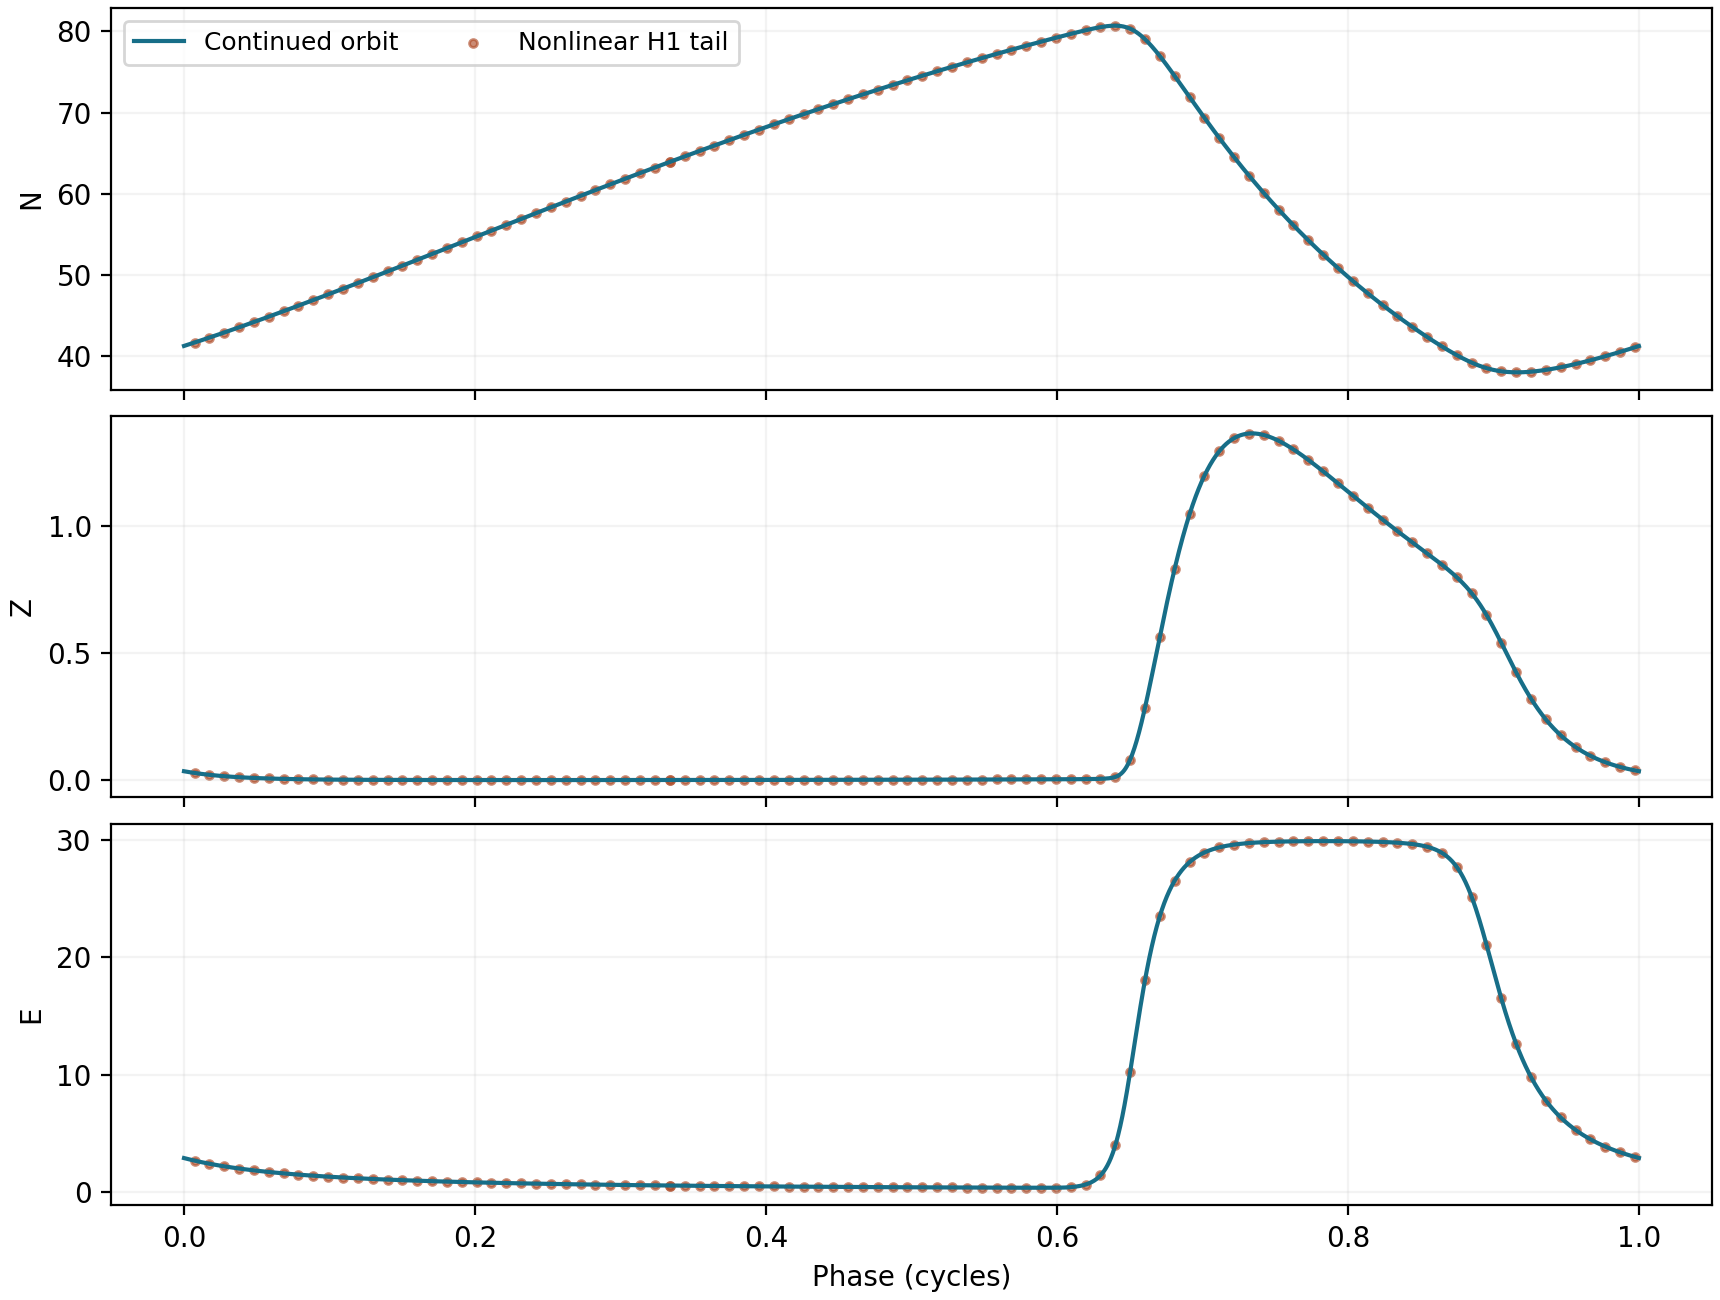
\includegraphics[width=0.9\textwidth,height=\textheight]{../figures/fig3_waveform_match_v42.png}
\caption{Figure S15. Continued orbit and independently integrated H1
tail at delay 149.5 years. The overlay uses one phase shift, with fixed
period and amplitudes.}
\end{figure}

\subsection{S16. Within-stock institutional-event
evidence}\label{s16.-within-stock-institutional-event-evidence}

\subsubsection{S16.1 Extraction and endpoint
protocol}\label{s16.1-extraction-and-endpoint-protocol}

The observational unit is a documented advice/action episode within
North Sea autumn-spawning herring, not a national aggregate. The
targeted source pair is Simmonds (2007), Table 1, pp.~688--689, and the
Cefas account by J.H. Nichols (1999), \emph{Saving North Sea herring}.
The first reconstructs historical ICES/NEAFC records; the second
supplies agency chronology for 1995--1996. The source pair was selected
to test temporal plausibility within the small-pelagic class. This is a
transparent retrospective extraction, not a preregistered or
representative sample.

Events are stored with separate advice, restrictive implementation,
closure and reopening labels in \texttt{institutional\_events\_v42.csv}.
A year has January 1--December 31 bounds; a month retains its first/last
dates. For a directed advice-to-action clock, interval subtraction
propagates precision and a causal lower bound of zero. The 1996 action
is constrained to follow the urgent May advice. This also tightens the
action lower bound for the October 1995 advice clock. Day differences
are divided by 365.25; displayed bounds are rounded outwards. Calendar
bounds are not confidence intervals. Multiple clocks sharing an action
or episode are dependent.

The 1965 general recommendation, 1970 specific TAC recommendation, 1976
first restrictive TAC and 1977 directed closure are extracted from the
separately typeset rows, not inferred from a figure. Nominal earlier TAC
agreements are not relabeled as restrictive implementation. The October
1995 and May 1996 advice events and implementation during 1996 are
separately recorded. No exact implementation day is assigned from the
date of a negotiation meeting. The general closure ending in 1983
remains a distinct endpoint; it is not pooled with reports of earlier
partial reopening or used as an advice-to-action delay.

The derived clocks are approximately \([10,12]\), \([5,7]\), \([6,8]\),
\([0.50,1.26]\) and \([0,0.67]\) yr with the definitions in the main
text. They constrain which historical clock is compatible with a
predicted time window. Five clocks from two episodes do not supply an
empirical governance-lag distribution or identify the model's constant
deployment delay. Post hoc overlap with the \(g=2\) window is a
compatibility check, not a fitted likelihood or prediction score.

\subsubsection{S16.2 Identification and the next dynamic
test}\label{s16.2-identification-and-the-next-dynamic-test}

A dynamic fishery test requires a stock observation operator (for
example, spawning biomass versus total renewable stock), a
unit-consistent effective-effort series, a separately measured
institutional response/process signal, recruitment and major
environmental covariates, and a specified response-law interpretation.
The transformation \(E\mapsto sE\), \(q\mapsto q/s\),
\(E_{\max}\mapsto sE_{\max}\), \(\delta_0\mapsto s\delta_0\) and
\(E_0\mapsto sE_0\) leaves \(N\), catch and the scaled model dynamics
invariant. Stock/catch data alone therefore cannot identify both effort
units and catchability.

The different TAC quantities in retrospective accounts are not pooled
without scope and assessment-vintage reconciliation. Spawning-stock
observations are not silently used as the model total stock. No plotted
series is digitized, no stock values are generated from projections, and
no event lag is entered as an observed DDE parameter. The present
evidence supports temporal discrimination within one stock, not dynamic
validation or global calibration. A prospective dynamic test should fix
its observation mapping and competing recruitment/environmental model
before estimation, separate training and evaluation periods, and
propagate process/observation uncertainty. The current package supplies
the endpoint data and exact model symmetries needed to make that test
identifiable rather than implying it has already been achieved.

\subsubsection{S16.3 Sources}\label{s16.3-sources}

Simmonds, E.J. (2007). Comparison of two periods of North Sea herring
stock management: success, failure, and monetary value. \emph{ICES
Journal of Marine Science} \textbf{64}, 686--692.
doi:10.1093/icesjms/fsm045. Publicly accessible source:
https://www.vliz.be/imisdocs/publications/222472.pdf .

Nichols, J.H. (1999). \emph{Saving North Sea herring}. Cefas, Lowestoft,
4 pp.~Agency publication record and account:
https://www.cefas.co.uk/data-and-publications/publications/list/publication-abstract/?id=12671
.

Hocherman, L., Trop, T., Ghermandi, A. (2025). Time lags in
environmental governance: A critical review. \emph{Ambio} \textbf{54},
2042--2059. doi:10.1007/s13280-025-02211-y. This heterogeneous synthesis
motivates endpoint care; it is not used as a 2--13-year empirical delay
distribution.

\end{document}
